\chapter{Reliability: Bias, Robustness, Privacy, and Safety}

\begin{learninggoals}
\item Understand reliability as a property of the full pipeline rather than only the trained model.
\item Explain how subgroup evaluation, robustness checks, privacy protections, and safety constraints all operationalize reliability.
\item Compute and interpret basic subgroup metrics such as accuracy, true positive rate, and false positive rate.
\item Distinguish distribution shift, spurious correlation, privacy leakage, and safety failure as different reliability problems.
\item Learn when a system should be redesigned, constrained, or rejected rather than simply tuned harder.
\end{learninggoals}

Chapter 11 argued that experimental results only matter when claims match evidence. Reliability extends that discipline into higher-stakes questions and turns it into a deployment constraint. It asks not only whether a model works on average, but for whom, under what shifts, with what privacy costs, and with what safety margins when failure matters. The chapter culminates in a reliability review card, so the early slice dashboards and harm models should be read as preparation for one launch decision rather than as a detached ethics checklist.

\begin{problemsolvinglens}
This chapter widens the seven-question framework from average performance to bounded failure. The question is no longer only ``does it work?'' but ``for whom, under what changes, and with what unacceptable risks?''
\end{problemsolvinglens}

\section{Reliability Is a Pipeline Property}

Every AI system simplifies reality. The question is not whether simplification occurs, but how its consequences are distributed and whether the resulting failures are acceptable. Reliability is therefore not a property that can be read off one model checkpoint. It emerges from data collection, labeling, measurement, representation, objective choice, thresholding, interface design, monitoring, and deployment context. This full-pipeline framing matches work that locates harm across the machine-learning life cycle rather than only in the final trained model \citep{suresh2021}.

This chapter groups together bias, robustness, privacy, and safety because they are often separated artificially in teaching. In practice they interact. A subgroup failure may be caused by data imbalance, but it may only become visible under a domain shift. A privacy mechanism may reduce memorization risk but also alter utility. A safety guardrail may depend on uncertainty estimation and fallback design. The unifying idea is that reliability means the system continues to behave within acceptable bounds under the conditions that matter.

\begin{decisionbox}
Do not ask only ``how accurate is the model?'' Ask ``for whom does it work, under what changes does it fail, what information might it expose, and what happens when it is wrong?'' Reliability begins when those questions become part of the core technical design.
\end{decisionbox}

\begin{practicalnote}
A compact reliability workflow is: name the harm model, identify operational slices, measure subgroup metrics, stress the system under realistic shifts, decide what fallback or no-launch condition is required, and then record that decision on the review card. The rest of the chapter fills in the evidence each step needs.
\end{practicalnote}

\begin{thinkingtool}
\textbf{Wrong question $\rightarrow$ better question.} Wrong: ``Is the model fair, robust, private, and safe?'' Better: ``For whom can it fail, under what shifts, what information might leak, and which failures are unacceptable enough to block deployment?''
\end{thinkingtool}

\begin{thinkingtool}
\textbf{Common failure mode $\rightarrow$ recovery move.} Failure mode: computing one fairness or robustness number, seeing that it looks acceptable, and stopping the review there. Recovery move: specify the harm model, evaluate operational slices separately, inspect severe failures directly, and tighten the fallback or redesign the pipeline when any subgroup or shift still faces unacceptable risk.
\end{thinkingtool}

\begin{thinkingtool}
\textbf{Signal to trust $\rightarrow$ signal to doubt.} Trust: the harm model is explicit, operational slices are reported separately, severe failures are inspected directly, and fallback or escalation paths are tightened where risk remains. Doubt: the system looks acceptable only in aggregate, subgroup or shift behavior is unreported, and privacy or safety is mentioned as a principle rather than reviewed as an operational failure channel.
\end{thinkingtool}

Keep one running case in view throughout this chapter: the grounded course-support assistant from the earlier language and experiments chapters. It routes student questions, retrieves policy passages, sometimes generates grounded answers, and sometimes escalates to humans. This case is useful because it looks ordinary enough to tempt careless deployment, yet it concentrates all four reliability themes in one pipeline: subgroup gaps in language coverage, robustness failures when wording or policy context shifts, privacy exposure through sensitive student records, and safety failures when the system answers questions that should have been escalated.

To keep the reliability story visibly cross-domain, this chapter also returns to the dashboard-camera pedestrian detector from Chapter 8. That contrast case moves the same ideas into sensor shift, bystander privacy, and bounded physical risk. The point is not that the domains are identical. It is that the same reliability questions survive domain change.

\begin{figure}[t]
\centering
\resizebox{\linewidth}{!}{\definecolor{biascolor}{rgb}{0.75,0.15,0.15}
\definecolor{robustcolor}{rgb}{0.15,0.50,0.75}
\definecolor{privacycolor}{rgb}{0.50,0.15,0.70}
\definecolor{safetycolor}{rgb}{0.10,0.60,0.20}

\begin{tikzpicture}[
    x=1cm, y=1cm,
    font=\small,
    %% Column centres:  x = 2.3  5.3  8.3  11.3   (cell width=3.0cm, pitch=3.0cm)
    %% Row centres:     y = 8.5  6.0  3.5   1.0   (row pitch=2.5cm)
    chdr/.style={draw=gray!50, fill=gray!15, rounded corners=2pt,
                 minimum width=3.0cm, minimum height=0.9cm,
                 text width=2.8cm, align=center, font=\footnotesize\bfseries},
    rhdr/.style={draw=gray!50, fill=gray!15, rounded corners=2pt,
                 minimum width=0.75cm, minimum height=2.5cm,
                 align=center, font=\footnotesize\bfseries, rotate=90},
    cell/.style={draw=gray!40, minimum width=3.0cm, minimum height=2.5cm,
                 text width=2.8cm, align=center, font=\footnotesize},
    bcell/.style={cell, fill=biascolor!10,    draw=biascolor!50},
    rcell/.style={cell, fill=robustcolor!10,  draw=robustcolor!50},
    pcell/.style={cell, fill=privacycolor!10, draw=privacycolor!50},
    scell/.style={cell, fill=safetycolor!10,  draw=safetycolor!50},
]

%% ── Title ────────────────────────────────────────────────────────────────
\node[font=\small\bfseries] at (6.4,11.0)
    {Reliability Evaluation Matrix: Full-Pipeline Assessment};

%% ── Column headers ───────────────────────────────────────────────────────
\node[chdr] at (2.3, 10.25)  {Data \&\\Labels};
\node[chdr] at (5.3, 10.25)  {Model \&\\Training};
\node[chdr] at (8.3, 10.25)  {Inference \&\\Decision};
\node[chdr] at (11.3,10.25)  {Deployment \&\\Monitor};

%% ── Row headers ──────────────────────────────────────────────────────────
\node[rhdr, fill=biascolor!15,    draw=biascolor]    at (0.375,8.5) {\textbf{BIAS}};
\node[rhdr, fill=robustcolor!15,  draw=robustcolor]  at (0.375,6.0) {\textbf{ROBUST.}};
\node[rhdr, fill=privacycolor!15, draw=privacycolor] at (0.375,3.5) {\textbf{PRIVACY}};
\node[rhdr, fill=safetycolor!15,  draw=safetycolor]  at (0.375,1.0) {\textbf{SAFETY}};

%% ═══════════════════════════════════════════════════════════════════════════
%% BIAS ROW  (y = 8.5)
%% ═══════════════════════════════════════════════════════════════════════════
\node[bcell] at (2.3,8.5)
    {\textbf{Representation}\\[2pt]
     Coverage gaps\\Label quality\\Annotation bias};

\node[bcell] at (5.3,8.5)
    {\textbf{Learning}\\[2pt]
     Objective imbalance\\Feature selection\\Group interactions};

\node[bcell] at (8.3,8.5)
    {\textbf{Allocation}\\[2pt]
     Unequal outcomes\\Service quality gaps\\Threshold effects};

\node[bcell] at (11.3,8.5)
    {\textbf{Operational}\\[2pt]
     Feedback loops\\Drift monitoring\\Harm detection};

%% ═══════════════════════════════════════════════════════════════════════════
%% ROBUSTNESS ROW  (y = 6.0)
%% ═══════════════════════════════════════════════════════════════════════════
\node[rcell] at (2.3,6.0)
    {\textbf{Distribution}\\[2pt]
     Domain coverage\\Shortcut risks\\Spurious patterns};

\node[rcell] at (5.3,6.0)
    {\textbf{Generalisation}\\[2pt]
     Regularisation\\Augmentation policy\\Hold-out domains};

\node[rcell] at (8.3,6.0)
    {\textbf{Shift Handling}\\[2pt]
     New conditions\\Edge cases\\Confidence scores};

\node[rcell] at (11.3,6.0)
    {\textbf{Adaptation}\\[2pt]
     Performance drift\\Graceful degradation\\Human handoff};

%% ═══════════════════════════════════════════════════════════════════════════
%% PRIVACY ROW  (y = 3.5)
%% ═══════════════════════════════════════════════════════════════════════════
\node[pcell] at (2.3,3.5)
    {\textbf{Collection}\\[2pt]
     Sensitive attributes\\Consent boundaries\\Retention policies};

\node[pcell] at (5.3,3.5)
    {\textbf{Training}\\[2pt]
     Memorisation risk\\Inference attacks\\Differential privacy};

\node[pcell] at (8.3,3.5)
    {\textbf{Output}\\[2pt]
     Information leakage\\Re-identification risk\\Output sanitisation};

\node[pcell] at (11.3,3.5)
    {\textbf{Lifecycle}\\[2pt]
     Log management\\Access controls\\Deletion schedules};

%% ═══════════════════════════════════════════════════════════════════════════
%% SAFETY ROW  (y = 1.0)
%% ═══════════════════════════════════════════════════════════════════════════
\node[scell] at (2.3,1.0)
    {\textbf{Assumptions}\\[2pt]
     Task boundaries\\World-model limits\\Scope validation};

\node[scell] at (5.3,1.0)
    {\textbf{Constraints}\\[2pt]
     Bounded outputs\\Adversarial robustness\\Red teaming};

\node[scell] at (8.3,1.0)
    {\textbf{Failure Modes}\\[2pt]
     Escalation triggers\\Abstention policies\\Worst-case analysis};

\node[scell] at (11.3,1.0)
    {\textbf{Operations}\\[2pt]
     Incident response\\Human oversight\\Kill switches};

%% ══════════════════════════════════════════════════════════════════════════
%% LEGEND
%% ══════════════════════════════════════════════════════════════════════════
\draw[gray!40] (0.75,-0.3) -- (12.8,-0.3);
\node[font=\footnotesize, text=green!55!black] at (2.3,-0.8)
    {\textbf{\checkmark}\ Acceptable risk};
\node[font=\footnotesize, text=orange!70!black] at (6.55,-0.8)
    {\textbf{!}\ Needs attention};
\node[font=\footnotesize, text=red!65!black] at (10.8,-0.8)
    {\textbf{$\times$}\ Blocks deployment};

%% ── Key insight ──────────────────────────────────────────────────────────
\node[draw=robustcolor!60, rounded corners=3pt, fill=robustcolor!8,
      minimum width=12.05cm, minimum height=0.85cm, align=center,
      font=\small] at (6.775,-1.6)
    {\textcolor{robustcolor!80!black}{\bfseries
     Each cell requires specific checks ---
     no single metric captures full reliability}};

\end{tikzpicture}
}
\caption{The reliability evaluation matrix shows that each reliability dimension (bias, robustness, privacy, safety) requires specific checks across every pipeline stage. No single metric captures full reliability—systematic assessment across all cells prevents deployment of systems with hidden failure modes.}
\label{fig:reliability-matrix}
\end{figure}

\section{Bias as a Full-Pipeline Failure}

Bias enters through many stages:
\begin{itemize}[leftmargin=*]
\item \textbf{data collection}: some groups or conditions are underrepresented
\item \textbf{labeling}: annotation quality differs across subpopulations
\item \textbf{measurement}: sensors or interfaces capture some groups less accurately
\item \textbf{representation}: useful distinctions for one group are blurred for another
\item \textbf{objective design}: optimizing one metric may hide unequal error patterns
\item \textbf{deployment}: a model is used in a setting unlike the one it was built for
\end{itemize}

This is why bias should not be treated as a moral adjective attached only to the model. It is a structured failure mode of the whole system.

\subsection{Harm Taxonomy Before Metrics}

Students often encounter reliability as a list of metrics and then try to choose one as if the metric itself decided the ethical and engineering question. That is backwards. The first step is to name the kind of harm that matters, because different harms require different evidence, different mitigations, and sometimes different system designs altogether.

A useful working taxonomy is:
\begin{itemize}[leftmargin=*]
\item \textbf{allocation harm}: the system grants or withholds opportunities unevenly, such as who receives a scholarship flag, a manual review, or a recommended intervention;
\item \textbf{quality-of-service harm}: the system serves some users less accurately, less clearly, or less reliably than others, even if the final binary decision looks similar;
\item \textbf{representation harm}: the system erases, stereotypes, or misdescribes people or groups in the language, labels, or categories it uses;
\item \textbf{privacy harm}: sensitive information is exposed, inferable, retained too long, or reused outside the justified purpose;
\item \textbf{safety or operational harm}: the system creates failures whose consequences are materially serious, such as bad medical triage, unsafe control behavior, or unbounded advice in a high-risk support context.
\end{itemize}

These categories overlap, but they are still useful because they keep the reliability review from collapsing into one vague fairness score. A course-support assistant might show quality-of-service harm for multilingual students, privacy harm if sensitive records leak into prompts or logs, and safety harm if high-risk messages are answered directly instead of escalated. One dashboard number cannot summarize all three responsibly.

\begin{practicalnote}
Ask ``what kind of harm are we trying to rule out?'' before asking ``which metric should we compute?'' Reliability metrics become more meaningful once the harm model is explicit.
\end{practicalnote}

\subsection{Overall Performance Can Hide Unequal Harm}

A system can achieve strong average metrics while failing badly for a subgroup. If the subgroup is small relative to the full dataset, the overall score may barely move even when the subgroup problem is severe. This is not a side issue. In many deployments, the subgroup may correspond to the most vulnerable, least represented, or most important users. Cases such as Gender Shades made this risk visible by showing large intersectional error gaps hidden inside commercial systems that might otherwise have looked acceptable in aggregate \citep{buolamwini2018}.

\begin{definition}[Subgroup Evaluation]
Subgroup evaluation measures model performance separately for distinct groups, conditions, or slices rather than only in aggregate.
\end{definition}

\subsection{A Subgroup Reliability Dashboard}

One fairness metric in isolation is rarely enough. A subgroup can look acceptable on accuracy while still receiving overconfident automation, too many unsafe direct answers, or too little human review. A better habit is to maintain a small subgroup dashboard that keeps several reliability questions visible at once.

For each operationally relevant subgroup, record at least:
\begin{itemize}[leftmargin=*]
\item sample size, so small groups are not overinterpreted or ignored;
\item task metric, such as accuracy, recall, or error rate for the decision that matters;
\item calibration or confidence quality, if confidence affects escalation or abstention;
\item abstention or escalation rate, if the system is allowed to defer;
\item severe-failure count, if some mistakes matter much more than others.
\end{itemize}

\begin{practicalnote}
Small slices are noisy. If a subgroup has only a few dozen examples, a one- or two-case change can move the metric materially. Treat large gaps as real signals, but treat small gaps on tiny slices as hypotheses until they survive more data or repeated evaluation.
\end{practicalnote}

This format matters because subgroup disparities do not always appear in the same column. One group may have similar accuracy but much worse calibration. Another may receive far more abstentions because the system is less certain, which may be a safe design choice or a service-quality problem depending on the application. Yet another may look fine on average while concentrating the worst errors in exactly the cases that should have triggered escalation.

\begin{decisionbox}
Do not ask only whether subgroup metrics are equal. Ask whether each subgroup receives an acceptable combination of accuracy, confidence quality, escalation behavior, and severe-failure exposure.
\end{decisionbox}

For the running support-assistant case, the dashboard might track dominant-register versus multilingual messages, routine policy questions versus high-risk escalation cases, and short messages versus long narrative messages. For the pedestrian detector, the analogous dashboard might track day versus night, dry versus wet conditions, and child versus adult pedestrian slices. The principle is the same: reliability review should compare operational slices with enough structure to reveal different failure channels, not just one averaged score per group.

\subsection{Worked Example: Accuracy Is Not the Whole Story}

Suppose the course-support assistant is evaluated on two groups of messages. Group A contains questions written in the dominant formal register well represented in training data. Group B contains questions written in a less represented informal or multilingual register.

For Group A:
\[
\text{TP}=45,\quad \text{FN}=5,\quad \text{FP}=10,\quad \text{TN}=40.
\]
For Group B:
\[
\text{TP}=8,\quad \text{FN}=12,\quad \text{FP}=2,\quad \text{TN}=18.
\]

Group A accuracy is
\[
\frac{45 + 40}{45 + 5 + 10 + 40} = \frac{85}{100} = 0.85.
\]
Group B accuracy is
\[
\frac{8 + 18}{8 + 12 + 2 + 18} = \frac{26}{40} = 0.65.
\]

Now consider the true positive rate:
\[
\mathrm{TPR} = \frac{\mathrm{TP}}{\mathrm{TP}+\mathrm{FN}}.
\]
Group A has
\[
\mathrm{TPR}_A = \frac{45}{45+5} = 0.90,
\]
while Group B has
\[
\mathrm{TPR}_B = \frac{8}{8+12} = 0.40.
\]

This is a much sharper picture than overall accuracy alone. If the task is routing students to the right policy or escalation path, the gap in true positive rate may matter more than the average score. A system that misses the right route for underrepresented language varieties is not merely slightly worse. It is less reliable for a specific slice of real users.

\begin{prereqbridge}
Accuracy counts all correct predictions equally. True positive rate isolates how often truly positive cases are detected. False positive rate isolates how often negative cases are incorrectly flagged. Different applications care about these errors differently.
\end{prereqbridge}

\subsection{Fairness Metrics Are Tools, Not Magic}

Fairness metrics such as subgroup accuracy, true positive rate, false positive rate, demographic parity, or equalized odds are useful because they force modelers to examine uneven behavior explicitly \citep{hardt2016}. But no single metric captures all relevant harms. Different applications justify different tradeoffs, and some fairness objectives conflict with one another when base rates differ.

\begin{advancednote}
Equalized odds asks whether groups have similar true positive and false positive rates. Demographic parity asks whether groups receive positive predictions at similar rates. These may conflict, which is one reason reliability work requires judgment rather than metric worship.

One compact way to see the tension is to write, for group $A=a$ with base rate $\pi_a=P(Y=1\mid A=a)$,
\[
P(\hat Y=1\mid A=a)=\mathrm{TPR}_a\,\pi_a+\mathrm{FPR}_a\,(1-\pi_a).
\]
If equalized odds holds across groups, then $\mathrm{TPR}_a$ and $\mathrm{FPR}_a$ are the same for each group, so different base rates $\pi_a$ still produce different positive-prediction rates. In that case, demographic parity usually cannot hold at the same time unless the groups have equal base rates or the classifier is trivial.
\end{advancednote}

\begin{example}[Real-World Callout: Aggregate Performance Hid Unequal Failure]
Buolamwini and Gebru showed that commercial gender-classification systems could look broadly capable while producing substantially higher error rates for darker-skinned women than for lighter-skinned men \citep{buolamwini2018}. That result is exactly why subgroup evaluation matters: an aggregate success story can coexist with a severe failure for a specific population. Fairness metrics such as equal opportunity or equalized odds do not remove the need for judgment, but they make this kind of uneven behavior visible enough to challenge a misleading average-case narrative \citep{hardt2016}.
\end{example}

\subsection{Calibration Gaps Can Also Be Reliability Gaps}

Reliability is not only about whether predictions are correct. It is also about whether confidence is interpretable. If a system produces confidence scores that are systematically too high for one subgroup, then the system can look equally accurate in aggregate while still being more dangerous for that subgroup in practice. Modern neural systems are often poorly calibrated by default, which means their stated confidence can be higher than their true correctness rate \citep{guo2017}.

This matters immediately in the running support-assistant case. Suppose the model attaches a confidence score to whether a message can be answered automatically or should be escalated. If messages written in a dominant formal register receive well-calibrated confidence but multilingual or distressed messages receive overconfident scores, then the same threshold can produce uneven harm even before the final answer is generated.

\begin{example}[Same Threshold, Different Reliability]
Imagine two groups of support messages. In Group A, messages scored at confidence $0.9$ are actually correct about $90\%$ of the time. In Group B, messages scored at confidence $0.9$ are correct only about $65\%$ of the time. A single confidence threshold may then look principled while silently exposing Group B users to much riskier automation. The engineering lesson is simple: reliability review should inspect calibration and threshold behavior by slice, not only global score distributions.
\end{example}

\begin{practicalnote}
If a model's confidence is used to decide escalation, triage, or human review, calibration becomes part of the system contract rather than a cosmetic diagnostic.
\end{practicalnote}

\section{Robustness Under Change}

\begin{definition}[Robustness]
Robustness is the ability of a model or system to continue behaving reasonably when inputs, environments, or usage conditions differ from the development setting.
\end{definition}

Robustness is not the same as average test accuracy. A model may perform well on one benchmark distribution and fail under small, predictable changes. This can happen because the model relied on shortcuts, because the representation is brittle, or because the deployment domain has shifted in ways the model never learned to handle. Benchmarks based on common corruptions made this problem concrete by evaluating the same classifier under systematic input degradation rather than only on clean test images \citep{hendrycks2019}.

\subsection{Common Forms of Shift}

Several reliability-relevant shifts appear repeatedly:
\begin{itemize}[leftmargin=*]
\item benign covariate shift such as lighting, microphone, or interface changes
\item subgroup-specific measurement degradation
\item domain shift across institutions, devices, or demographics
\item wording or policy shift after a new semester, new interface, or updated documentation
\item adversarial perturbation intended to trigger failure
\item concept drift, where the task itself changes over time
\end{itemize}

\subsection{Spurious Correlations}

Many robustness failures are caused by spurious correlations. A model learns a pattern that predicts well in training but is not the intended signal. Snow in wolf photos, scanner artifacts in medical data, room acoustics in keyword detection, or formatting quirks in text can all become accidental shortcuts. In a support assistant, a model may over-rely on course codes, platform names, or the phrasing habits of one institution rather than on the underlying request. The system may appear successful until the spurious cue disappears.

Figure~\ref{fig:zech-domain-shift} gives a concrete hospital-shift example from chest-radiograph modeling. In the original study, MSH refers to Mount Sinai Hospital and NIH refers to the NIH ChestXray dataset. As the relative pneumonia prevalence changes across those sources, internal and external performance move in different directions. That is exactly what shortcut learning under domain shift looks like: the model appears to improve under one validation story while becoming less reliable under the deployment-relevant one.

\begin{figure}[t]
\centering
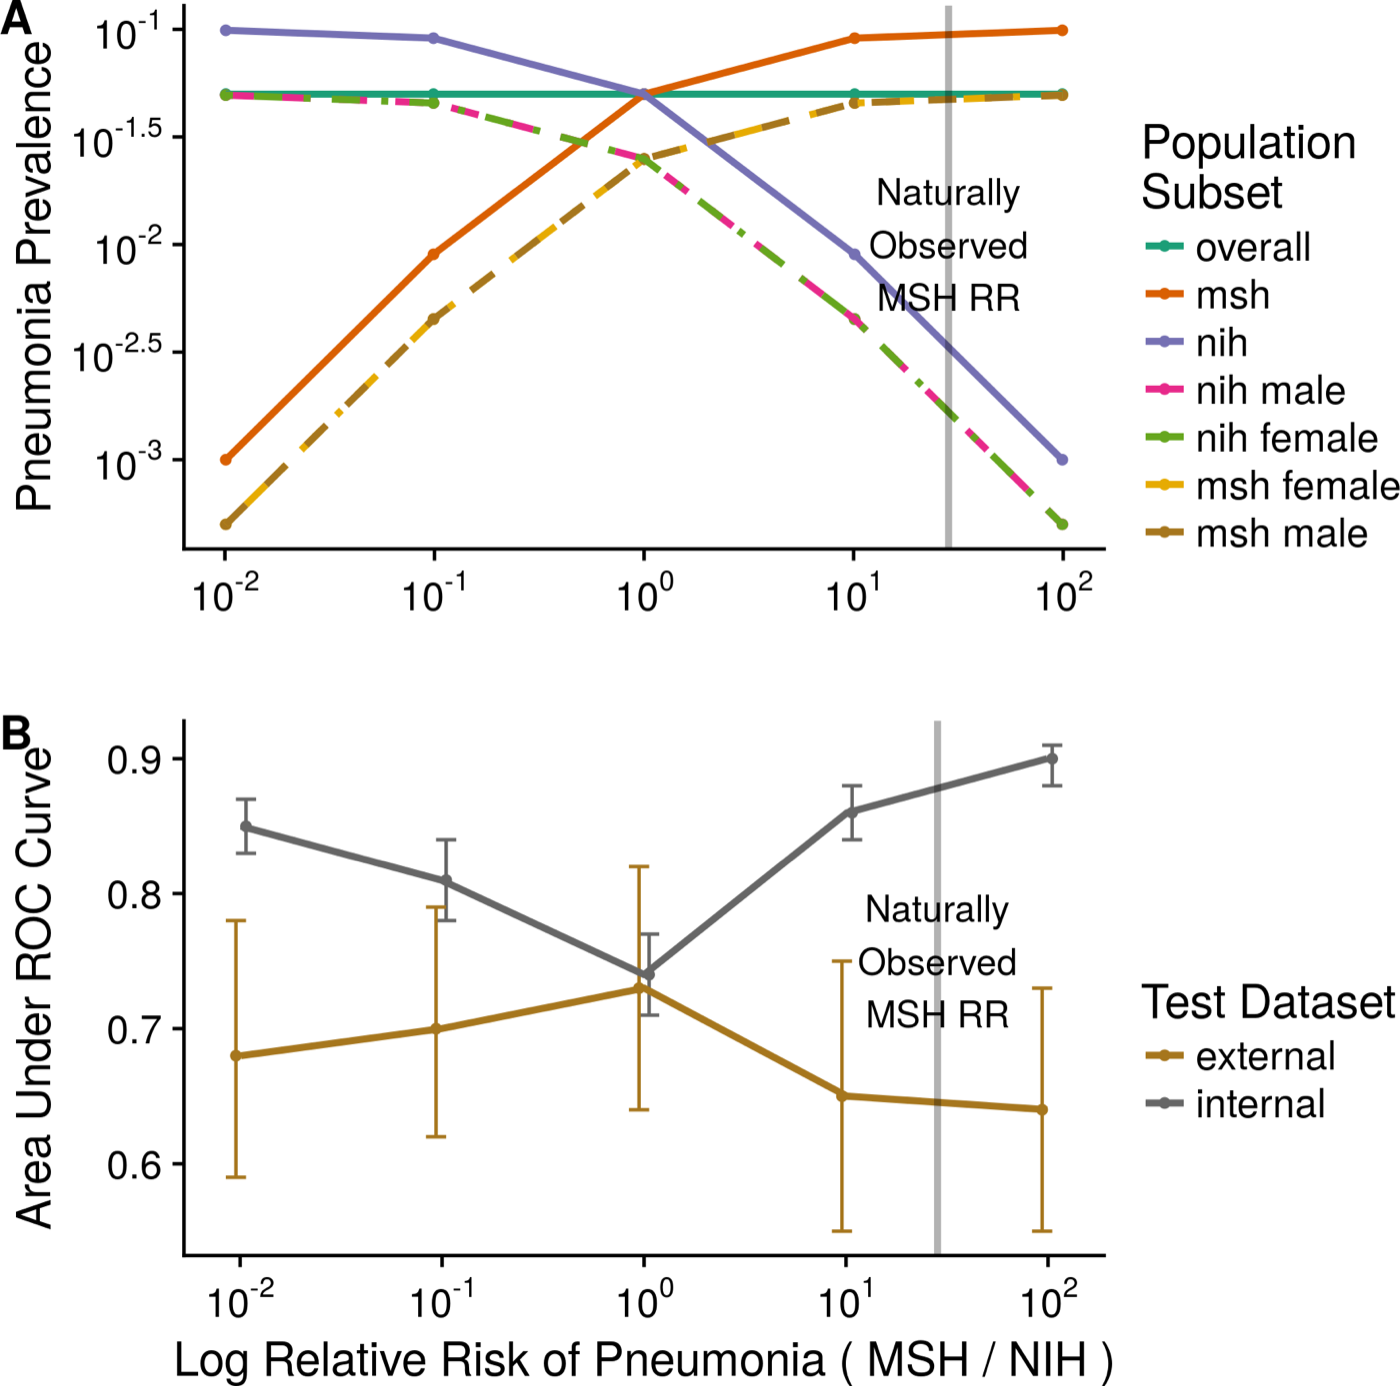
\includegraphics[width=0.72\linewidth]{figures/external/zech2018_g003_small.png}
\caption{Institutional shift can reverse the story told by internal validation. In this open-access figure from \citet{zech2018}, internal AUC and external AUC diverge as the relative pneumonia prevalence between hospital sources changes. Reproduced from a PLOS Medicine article distributed under CC BY 4.0.}
\label{fig:zech-domain-shift}
\end{figure}

\begin{failurebox}
Reliability failures often look like competence until the environment changes. This is why a clean benchmark can be misleading: it may reward shortcut use instead of robust understanding of the intended task.
\end{failurebox}

\subsection{Worked Example: A Reliability Tradeoff}

Suppose a course-support assistant is evaluated under two conditions:
\begin{itemize}[leftmargin=*]
\item familiar wording from the current semester's policies and student messages
\item shifted wording from a new semester, with revised policy language and more varied student phrasing
\end{itemize}
Across repeated runs, a baseline support model achieves mean familiar-wording accuracy about $0.914$ but mean shifted-wording accuracy only about $0.627$. After adding paraphrase augmentation and more diverse retrieval-side query rewriting during training, the model's mean familiar-wording accuracy drops to about $0.892$ but shifted-wording accuracy rises to about $0.812$.

This is a reliability result, not merely an accuracy result. The right claim is not that augmentation is universally better. It is that the new training procedure improves robustness to the specific wording shift of interest while trading away some performance on the familiar slice. Reliability often lives in these tradeoffs.

\subsection{Stress Tests Should Be Designed, Not Improvised}

Robustness evaluation becomes much stronger once teams name the changes they actually expect in deployment and test them deliberately. For image models, this may mean blur, noise, corruption, compression artifacts, weather, or camera shift. For language systems, it may mean paraphrase, spelling variation, multilingual phrasing, outdated policy pages, or retrieval-index changes. Benchmarks based on common corruptions became influential precisely because they turned vague robustness talk into a repeatable stress protocol \citep{hendrycks2019}.

\begin{table}[t]
\centering
\small
\setlength{\tabcolsep}{4pt}
\begin{tabular}{p{2.91cm}p{3.07cm}p{3.96cm}}
\toprule
System type & Stress scenario & What the test is trying to reveal \\
\midrule
Course-support assistant & paraphrased or multilingual student phrasing & whether routing and retrieval depend too heavily on familiar lexical forms \\
Course-support assistant & updated policy page structure or terminology & whether retrieval and answer generation stay grounded after document drift \\
Pedestrian detector & night rain, glare, or new camera placement & whether visual competence relies on familiar conditions rather than robust cues \\
Forecasting system & delayed sensor updates or seasonal regime change & whether the model has learned stable signal or only local historical regularities \\
\bottomrule
\end{tabular}
\caption{Stress tests are more informative when they are named in advance and tied to realistic deployment changes rather than chosen after failure is observed.}
\label{tab:reliability-stress-tests}
\end{table}

The chapter's broader lesson is that robustness tests should be justified by a deployment story. A benchmark corruption that never appears in practice may still be pedagogically useful, but the strongest reliability evidence comes from changes that the system is actually likely to face.

\section{Privacy as a Modeling Constraint}

Privacy is not merely a legal layer added after technical work. It shapes what data may be collected, stored, linked, and learned from in the first place.

In the running support-assistant case, this point becomes immediate. Student messages may mention illness, disability accommodations, visa status, financial hardship, grade disputes, or identifying numbers. A team that casually logs and reuses such messages for model improvement may create privacy risk long before deployment decisions become visible.

The vision contrast case makes the same point differently. Dashboard-camera footage can capture faces, license plates, home addresses, and repeated movement patterns of bystanders who never consented to becoming training data. A perception task that seems less personal than text can still create serious privacy exposure if collection, retention, or reuse rules are weak.

\subsection{Privacy Threat Models Before Privacy Tools}

Privacy review improves once it stops asking only ``which protection should we use?'' and starts asking ``who could learn what, through which access path, and with what consequence?'' That is a threat-model question. Without it, privacy discussion can become a vague checklist of fashionable defenses rather than an engineering analysis of actual exposure.

A compact privacy threat model names:
\begin{itemize}[leftmargin=*]
\item \textbf{the sensitive asset}: what information must be protected, such as health disclosures, identifiers, location traces, or accommodation status;
\item \textbf{the attacker or observer}: who might gain access, such as internal reviewers, external users, data brokers, compromised services, or other institutions;
\item \textbf{the access path}: logs, prompts, retained training data, retrieval indexes, debugging tools, model outputs, or linkage across datasets;
\item \textbf{the consequence}: embarrassment, discrimination, financial loss, legal exposure, or physical risk.
\end{itemize}

For the support-assistant case, one threat model might say: sensitive student records and messages are the asset; internal debugging access and long-lived prompt logs are the path; unauthorized staff or compromised tooling are the observer; and the consequence is exposure of disability, immigration, or health information. For the pedestrian-detector case, the asset may be identifiable faces or movement patterns; the path may be retained video and annotation tooling; and the consequence may be long-term surveillance or unconsented secondary use.

\begin{decisionbox}
Before choosing a privacy method, write one sentence of the form: ``We are trying to stop \emph{this observer} from learning \emph{this sensitive fact} through \emph{this data path}.'' If that sentence is vague, the privacy design is probably vague too.
\end{decisionbox}

\subsection{Why Models Can Leak Information}

Training data may contain names, messages, health records, locations, or other sensitive content. A model can leak such information by memorizing rare examples, exposing hidden attributes through inference, or enabling linkage across datasets. Even if the model is not explicitly designed to reveal private information, its outputs or internals may still create privacy risk.

\subsection{Common Privacy Responses}

Several technical responses are common:
\begin{itemize}[leftmargin=*]
\item \textbf{data minimization}: collect and retain only what is necessary
\item \textbf{access control and secure storage}: reduce unnecessary exposure
\item \textbf{differential privacy}: constrain what the model can reveal about any individual example
\item \textbf{federated or distributed learning}: keep raw data decentralized in some workflows
\item \textbf{redaction and filtering}: remove especially sensitive fields before modeling
\end{itemize}

\subsection{Privacy Has Tradeoffs}

These techniques are not free. Stronger privacy constraints can reduce utility, increase computation, or complicate debugging. But that tradeoff is part of the real engineering problem. A system that performs well only by exposing people to unacceptable privacy risk is not a reliable system in any serious sense.

\begin{advancednote}
Differential privacy gives a formal guarantee that the output distribution of an algorithm changes only slightly when one training example is added or removed \citep{dwork2006}. The precise definition is more advanced than this chapter requires, but the intuition is important: privacy can be formalized as a bound on how much an individual's data can influence the released result.

Formally, a randomized mechanism $M$ is $\epsilon$-DP if for all neighboring datasets $D,D'$ and all events $S$,
\[
P(M(D)\in S)\le e^\epsilon P(M(D')\in S).
\]
A useful undergraduate intuition is sensitivity: if a query $q$ changes by at most $\Delta q$ when one record changes, then adding noise on the order of $\Delta q/\epsilon$ makes any single person's contribution hard to detect while preserving the coarse signal.
\end{advancednote}

\subsection{Privacy Risk Lives in the Whole Data Path}

Privacy review should follow the data path end to end:
\begin{itemize}[leftmargin=*]
\item what raw fields are collected,
\item what fields are joined or linked later,
\item what gets logged during inference,
\item who can inspect those logs,
\item what examples are retained for future training,
\item what generated outputs might reveal or reconstruct.
\end{itemize}

This framing helps students avoid a common mistake. They imagine privacy as a property of the final model weights alone. In real systems, the privacy risk may be dominated by preprocessing dumps, support logs, annotation tools, cached prompts, or debugging traces rather than by the final deployed checkpoint.

\begin{example}[A Privacy Failure Without an Exotic Attack]
A support assistant may never explicitly emit a student's name in the final answer yet still create serious privacy exposure if raw messages containing health details and accommodation requests are retained in accessible logs for prompt debugging. That is a systems failure, not only a modeling failure. The safest model architecture in the world will not repair careless retention and access rules.
\end{example}

\section{Safety and Bounded Failure}

Safety becomes especially important when AI systems influence high-stakes decisions, interact with the physical world, or generate open-ended outputs that can trigger harmful actions.

\begin{definition}[Safety]
Safety concerns whether a system's failures are anticipated, bounded, monitored, and handled in ways that keep harms within acceptable limits.
\end{definition}

This is broader than model accuracy. A medical triage assistant, an autonomous-driving perception module, and a general-purpose language assistant each face different safety problems. But they share a systems lesson: safety depends on fallback behavior, monitoring, escalation paths, human review, and clear operational limits.

The course-support assistant is a useful reminder that safety is not limited to robots or hospitals. A confident answer about visa attendance, disability accommodation, self-harm disclosures, or disciplinary policy can still create severe harm if the system answers when it should have escalated.

\begin{example}[Contrast Case: Safety in a Perception System]
Suppose a shuttle's pedestrian detector looks strong on familiar daylight footage but misses close-range pedestrians in headlight glare or night rain. The safety problem is not captured by average detection quality alone. It also depends on whether the vehicle slows down, hands control back to a human, or triggers a conservative fallback whenever visibility or model confidence becomes poor.
\end{example}

\subsection{Hazards, Not Just Errors}

An error becomes a safety issue when the consequences matter. Misclassifying one image in a photo app is not the same as missing a critical pathology finding. Safety analysis therefore begins by identifying hazards:
\begin{itemize}[leftmargin=*]
\item what types of error are possible?
\item which of them are severe?
\item how likely are they?
\item what mitigations reduce their impact?
\end{itemize}

\subsection{Safety Cases Make Bounded Failure Concrete}

Once hazards are named, the next step is to write a small safety case. The point is not to imitate a certification bureaucracy. It is to force the team to connect hazard, trigger, mitigation, fallback, and monitoring in one coherent argument.

A lightweight safety case can be written with five fields:
\begin{itemize}[leftmargin=*]
\item \textbf{hazard}: what harmful failure must be bounded;
\item \textbf{trigger condition}: under what inputs, environments, or uncertainty patterns the hazard is likely to appear;
\item \textbf{mitigation}: what model-side or pipeline-side design reduces the chance of that failure;
\item \textbf{fallback}: what the system does instead when the hazard cannot be ruled out confidently;
\item \textbf{monitoring signal}: what evidence after launch would indicate that the safety case is weakening.
\end{itemize}

For the course-support assistant, one safety case might center on high-risk student messages being answered directly when they should be escalated. The trigger condition could be a message that mixes routine academic language with distress, immigration, disability, or disciplinary cues. The mitigation could include high-risk intent detection, retrieval grounding, and conservative escalation thresholds. The fallback is immediate routing to trained human support. The monitoring signal is any rise in escalation misses or unsafe direct answers on audited high-risk slices.

For the pedestrian detector, the same pattern appears in another domain: the hazard is a missed close-range pedestrian; the trigger condition is glare, rain, or unusual night geometry; the mitigation is stress-tested sensing and conservative policy thresholds; the fallback is slowdown or human takeover; the monitoring signal is rising miss rate under those visibility conditions. The lesson is the same in both domains. Safety is strongest when failure handling is specified before deployment rather than improvised after the first incident.

\begin{evidencebox}
``The model is accurate'' is not a safety case. A safety case must say what the dangerous failure is, when it is likely, what reduces it, how the system falls back, and what signal would warn the team that the protection is no longer holding.
\end{evidencebox}

\subsection{Human Oversight and Fallbacks}

Some systems should assist rather than automate. A model may provide ranked options, highlight uncertainty, or request human confirmation when confidence is low or context is unusual. In other settings, rule-based guardrails or conservative thresholds may be more important than squeezing out another percentage point of average performance.

\begin{example}[A Safety Failure in an Ordinary Support System]
Suppose a student writes a message that mixes deadline language with a severe personal-risk signal or an immigration-status concern. A superficially competent assistant might answer only the visible deadline question because that is what the lexical content most strongly resembles. A safer system would route the message to a human support path, attach the relevant policy information, and decline to answer beyond its authority.
\end{example}

\subsection{Selective Automation Requires Usable Uncertainty}

Reliability often improves not by forcing the model to answer everything, but by giving it permission to abstain on the cases it does not understand well enough. Selective classification makes this logic explicit: the system chooses when to predict and when to defer, trading coverage against risk \citep{geifman2017}. Closely related ideas such as conformal prediction aim to provide uncertainty sets or calibrated coverage guarantees rather than one forced point prediction \citep{shafer2008}.

If a selector is $c(x)\in\{0,1\}$, where $c(x)=1$ means "answer," then coverage is
\[
\phi=\mathbb{E}[c(X)] \approx \frac{1}{n}\sum_{i=1}^n c_i,
\]
and selective risk is
\[
R_{\mathrm{sel}}=\frac{\sum_{i=1}^n c_i\,\ell_i}{\sum_{i=1}^n c_i},
\]
the average loss only on answered cases. A simple threshold rule makes the tradeoff concrete: answer only when $\max_k p(y=k\mid x)\ge \tau$. Higher $\tau$ usually lowers coverage but also lowers selective risk because the system abstains on harder examples.

This does not mean every application needs advanced uncertainty machinery. The operational lesson is more basic. If the system will be trusted differently at confidence $0.55$ and $0.95$, then confidence quality matters. Calibration, abstention rules, and human review thresholds become central parts of the reliability design rather than optional research extras.

\begin{decisionbox}
When the cost of a confident mistake is high, do not ask only how to improve the prediction. Ask how to make low-confidence or unfamiliar cases fall out of automation gracefully.
\end{decisionbox}

\begin{example}[Coverage Versus Safety]
Suppose the support assistant can answer $82\%$ of incoming questions automatically with very low factual error when it abstains on low-confidence or high-risk cases, but reaches $96\%$ automation only by answering many uncertain messages directly. The second system may look more efficient, yet the first may be far more reliable because its failures are bounded by design. The same principle appears in perception systems that slow down, request takeover, or switch to a conservative fallback when visibility is poor.
\end{example}

\begin{evidencebox}
Evidence for safety should include more than nominal test performance. It should include severe-failure analysis, operating thresholds, fallback behavior, monitoring plans, and documentation of what the system is \emph{not} intended to do.
\end{evidencebox}

\subsection{Reliability Is Sometimes a Reason to Decline Deployment}

This is an important professional lesson. Some systems should not be deployed yet. If subgroup failures are severe, privacy risks are unacceptable, or fallback behavior is missing in a high-stakes setting, the correct action may be to redesign the system or refuse deployment. Reliability is not only about mitigation. It is also about knowing when the evidence is not good enough.

\section{Monitoring Reliability After Launch}

Reliability does not end when the model leaves the notebook. Post-deployment monitoring is where many apparently careful systems begin to fail. User populations change, document collections drift, sensors degrade, labels arrive late, and human reviewers work under different load than anticipated. A system that was reliable at launch can become unreliable quietly unless the team watches the right signals.

For the running support-assistant case, useful monitoring signals might include subgroup routing accuracy, retrieval success on current policy passages, escalation miss rate on high-risk messages, citation coverage for grounded answers, and sudden changes in the distribution of incoming questions. For the pedestrian detector, useful signals might include weather-conditioned miss rates, takeover frequency, latency spikes, or changes in camera installation geometry.

\begin{thinkingtool}
\textbf{Monitoring question.} For every major reliability risk named before launch, specify one observable post-launch signal that would warn the team early if that risk were getting worse.
\end{thinkingtool}

Monitoring also connects directly to rollback and narrowing decisions. If a support assistant begins failing after a policy-site redesign, the right response may be to disable direct answers temporarily and revert to retrieval-plus-escalation. If a perception module shows degraded performance under a new camera firmware version, the right response may be to reduce automation authority until the shift is understood. A reliable system is therefore not just one that works initially. It is one whose failure can be noticed and bounded before harm compounds.

\section{Why Ethics and Engineering Cannot Be Separated}

One common mistake in AI education is separating ethics from engineering so completely that students discuss harms in one room and technical design in another. That structure quietly teaches the wrong lesson. It suggests that fairness, privacy, and safety are optional reflections added after the real work.

A better educational pattern is to show that:
\begin{itemize}[leftmargin=*]
\item subgroup metrics are technical measurements,
\item robustness tests are experimental design,
\item privacy protection constrains data and training,
\item safety analysis shapes thresholds and system architecture,
\item documentation and human oversight are engineering choices.
\end{itemize}

Ethical reflection remains broader than these tools, but reliability work is one place where ethical obligations become operational technical practice.

\section{Chapter Artifact: A Reliability Review Card}

By the end of Chapter 12, the reader should be able to produce a one-page reliability review card before saying a system is ready for serious use.

\begin{table}[t]
\centering
\small
\setlength{\tabcolsep}{4pt}
\begin{tabular}{p{3.25cm}p{6.98cm}}
\toprule
Review field & What must be written clearly \\
\midrule
Seven-question focus & Questions 3, 6, and 7 most directly: what data and deployment conditions create risk, what evidence bounds failure, and what review or fallback keeps the system acceptable \\
Critical users or slices & Which groups, contexts, or operating conditions must be checked separately \\
Shift scenarios & Which realistic changes in device, environment, source, or user population could break the system \\
Spurious-cue or measurement risks & What accidental shortcuts or measurement failures may be carrying the score \\
Privacy threat model & What sensitive fact is being protected, from whom, through which data path \\
Severe hazards & Which failures are unacceptable even if overall metrics stay strong \\
Safety case & For each severe hazard: trigger condition, mitigation, fallback, and monitoring signal \\
Fallback and review path & What abstention, escalation, or human-review route exists when the system is uncertain or high risk \\
Monitoring triggers & What post-deployment signals would indicate reliability degradation \\
No-deploy condition & What finding would be strong enough to delay, narrow, or reject deployment \\
\bottomrule
\end{tabular}
\caption{A reliability review card turns fairness, robustness, privacy, and safety into one bounded-failure protocol rather than four disconnected checklists.}
\label{tab:reliability-review-card}
\end{table}

\begin{thinkingtool}
\textbf{Reliability review card.} Before calling a system reliable, write down the critical slices, shift scenarios, privacy exposures, severe hazards, fallback path, monitoring triggers, and the condition under which deployment should be delayed or refused.
\end{thinkingtool}

\begin{example}[Filled Reliability Review Card]
For the course-support assistant, a disciplined review card would name critical slices such as multilingual phrasing, underrepresented language registers, visa-related questions, disability-accommodation requests, and distressed student messages; shift scenarios such as a new semester, revised syllabus wording, new learning-platform terminology, or policy-page reorganization; spurious cues such as course codes or standard-form wording that may not survive outside the training setting; privacy exposures such as student identifiers, health disclosures, and accommodation records; severe hazards such as answering high-risk questions directly when escalation is required; fallback path as human advising or specialist support teams; monitoring triggers as subgroup degradation, retrieval failures on policy pages, or rising escalation misses; and a no-deploy condition such as unacceptable failure on high-risk slices even when overall metrics remain strong.
\end{example}

\section{Common Mistakes in Reliability Work}

These mistakes are surface forms of the chapter's main enemy: confusing improved scores with justified explanation. Read them as one reliability checklist rather than five separate mini-topics.

\begin{mistakebox}
\item \textbf{Reporting only overall metrics.} Overall numbers can hide subgroup failures and robustness weaknesses.
\item \textbf{Treating bias as only a dataset issue.} Bias can enter through labels, measurements, thresholds, deployment conditions, and user interaction.
\item \textbf{Confusing robustness with clean accuracy.} A model may be accurate on a benchmark and brittle under predictable shift.
\item \textbf{Treating privacy as an afterthought.} Late privacy fixes are often expensive or insufficient.
\item \textbf{Thinking safety is just the model's job.} Fallback logic, escalation, monitoring, and interface design often matter more than one extra point of accuracy.
\end{mistakebox}

\section{Looking Ahead}

This chapter treated reliability as an engineering discipline across the full pipeline. The final chapter asks the launch question that follows from that discipline: once contracts, monitoring, fallback behavior, and ownership are included, is the whole system actually ready to operate as a real service?

\begin{chaptersummary}
\item Reliability is a property of the full pipeline, not just the trained model.
\item Subgroup evaluation is necessary because overall metrics can conceal unequal failures.
\item Fairness metrics such as accuracy, true positive rate, and false positive rate provide useful but incomplete views of reliability.
\item Robustness concerns how performance changes under realistic shift, noise, shortcut failure, or concept drift.
\item Privacy constrains what data can be used and what the model is allowed to reveal.
\item Safety depends on bounded failure, fallback behavior, monitoring, and human oversight.
\item Reliability is where ethical obligations and technical design become inseparable in practice.
\item The main deliverable of the chapter is a reliability review card that makes bounded-failure evidence explicit before deployment claims are made.
\end{chaptersummary}

\begin{studyquestions}
\item Why should bias be treated as a property of the full pipeline rather than only the model?
\item Why can subgroup true positive rate matter more than overall accuracy in some applications?
\item How is robustness different from average test performance?
\item Why does privacy count as a modeling constraint rather than only a policy issue?
\item What makes an error a safety issue rather than only a performance issue?
\item Why can refusing deployment be the correct reliability decision?
\item Why might a support assistant with good average performance still be unreliable on the questions that matter most?
\end{studyquestions}

\begin{exercises}
\item Compute the true positive rate and false positive rate for a small confusion matrix of your own design.
\item Give one example of a subgroup failure that could be hidden by a strong overall metric.
\item Describe one realistic spurious correlation for a vision, language, or audio task.
\item Explain one case in which a privacy-preserving design choice might reduce raw utility but still improve the overall system.
\item Give one example of a model that should assist a human rather than automate the decision completely.
\item Describe a deployment situation in which robustness to distribution shift matters more than clean benchmark accuracy.
\item For a support assistant or a dashboard-camera pedestrian detector, list one subgroup slice, one shift scenario, one privacy exposure, and one severe hazard that should appear on the reliability review card.
\item Use Table~\ref{tab:reliability-review-card} to sketch a one-page reliability review card for a system of your choice. If you are carrying one case through the book, write it for the same system as your experiment claim sheet and state which empirical claim survives this reliability review unchanged.
\end{exercises}

\begin{challengeexercises}
\item A classifier has similar overall accuracy across two groups but very different false positive rates. Explain why this can still be a serious reliability concern, and give a domain in which it would matter.
\item A team proposes deploying a model with excellent benchmark results but no subgroup analysis, no privacy review, and no fallback behavior. Write the strongest technical objection you can in one paragraph.
\item Compare two mitigation strategies for a minority-group performance gap: collecting better data versus threshold adjustment. Explain when each might help, what it cannot fix, and what evidence would be needed to judge it.
\end{challengeexercises}
